\documentclass[10pt, a4paper]{article}

%\usepackage[margin=2.5cm,nohead]{geometry}
%\renewcommand{\baselinestretch}{1.2} % mudar o espaçamento entre linhas
\usepackage[portuguese]{babel}
\usepackage{indentfirst}
\usepackage[utopia]{mathdesign}     % fonte Utopia para o documento inteiro
\usepackage{inconsolata}            % fonte mono-espaçada
\usepackage[stretch=10]{microtype}  % ajuste de espaçamento entre caracteres
\usepackage{hyperref}               % referências clicáveis
\usepackage{float}                  % posicionamento de figuras
\usepackage{lastpage}               % colocar última página no rodapé
%\usepackage{enumitem}               % modificar listagens
\usepackage{amsmath}                % escrita matemática
\usepackage[extreme]{savetrees}     % aproveitar espaço em branco


\usepackage{multicol}               % múltiplas colunas
\setlength{\columnsep}{1cm}

\usepackage{xcolor}     % mudar a cor do texto
\definecolor{uminho}{RGB}{150, 33, 24}
\definecolor{um_eng}{RGB}{173, 66, 15}

\usepackage{graphicx}     % inserir imagens
\graphicspath{{images/}}  % pasta das imagens

\usepackage{sectsty}          % personalizar capítulos/secções
\chapterfont{\color{uminho}}  % mudar cor dos capítulos
\sectionfont{\color{uminho}}  % mudar cor das secções
 
\usepackage{listings}
\lstset{basicstyle=\footnotesize\ttfamily,breaklines=true,keywordstyle=\color{um_eng}}

%\usepackage{todonotes}              % lista de to-dos
%\setlength{\marginparwidth}{2.5cm}  % tamanho das margens (para to-dos)

\setlength{\parskip}{0.2em}         % espaçamento entre parágrafos



\begin{document} 
\begin{multicols}{2}

\begin{center}
    \fbox{\textbf{\Large Formulário MDIO 2020/2021}}
\end{center}

\thispagestyle{empty}



\section{\texttt{Relax4}}

\subsection{Formato do input}

\begin{lstlisting}
n
m
org dst custo cap (m vezes)
vert (n vezes)
\end{lstlisting}

\begin{itemize}
    \item \textbf{\texttt{n}}: número de vértices
    \item \textbf{\texttt{m}}: número de arcos do grafo
    \item \textbf{\texttt{org}}: vértice de origem do arco
    \item \textbf{\texttt{dst}}: vértice de destino
    \item \textbf{\texttt{custo}}: custo de transporte
    \item \textbf{\texttt{cap}}: capacidade do arco
    \item \textbf{\texttt{vert}}: oferta/procura no vértice, \(+\) e \(-\) respetivamente
\end{itemize}



\section{Transportes: Introdução}

\subsection{Modelo geral}

\begin{figure}[H]
    \centering
    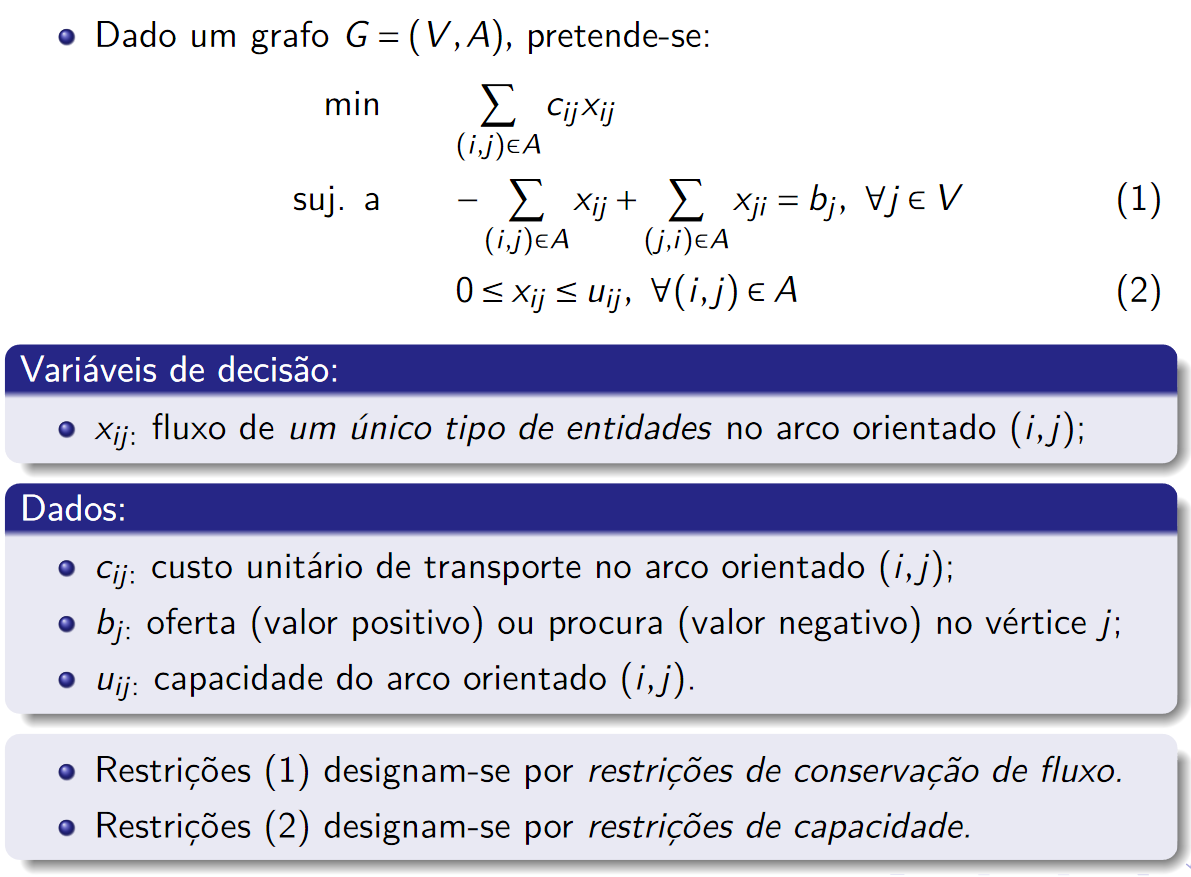
\includegraphics[width=0.45\textwidth]{modelo_geral_transportes.png}
\end{figure}

\subsection{Caracterização das soluções básicas}

A uma base podemos associar uma árvore (grafo com vértices não orientados) que suporta todos os vértices.

\subsubsection{Propriedades da árvore de suporte de um grafo G = (V, A)}

\begin{itemize}
    \item é um grafo ligado (existe um caminho entre cada par de vértices)
    \item sem ciclos
    \item com \(|A| = |V| - 1\) (nº de arcos = nº de vértices - 1)
\end{itemize}

\subsection{Método dos multiplicadores}

\begin{enumerate}
    \item Fixar o valor de qualquer multiplicador em 0
    \item Arcos básicos: \(c_{ij} = u_i - u_j\)
    \item Arcos não-básicos: $\delta_{ij} = c_{ij} - (u_i - u_j)$
\end{enumerate}

\subsection{Pivô}

\begin{figure}[H]
    \centering
    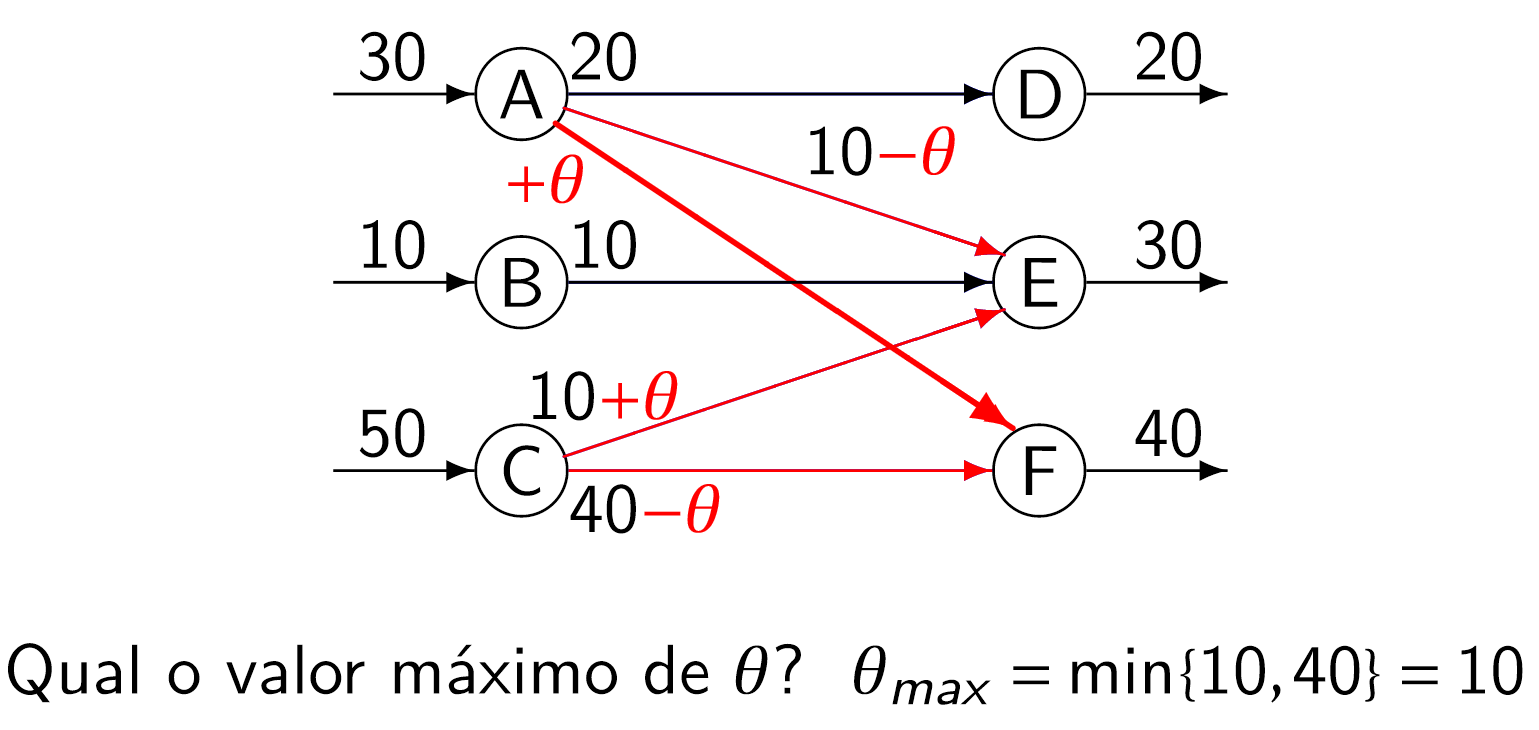
\includegraphics[width=0.35\textwidth]{pivo_intr.png}
\end{figure}



\section{Transportes: Grafos Bipartidos}

Um grafo \(G = (V, A)\) é bipartido se o conjunto de vértices \(V\) puder ser dividido em dois conjuntos disjuntos, \(V_1\) e \(V_2\) (i.e., \(V_1 \cup V_2 = V, V_1 \cap V_2 = \emptyset\)), de tal modo que todos os arcos \((i,j) \in A\) tenham origem num vértice \(i \in V_1\) e destino num vértice \(j \in V_2\).

%\subsection{Representações}
%
%\begin{figure}[H]
%    \centering
%    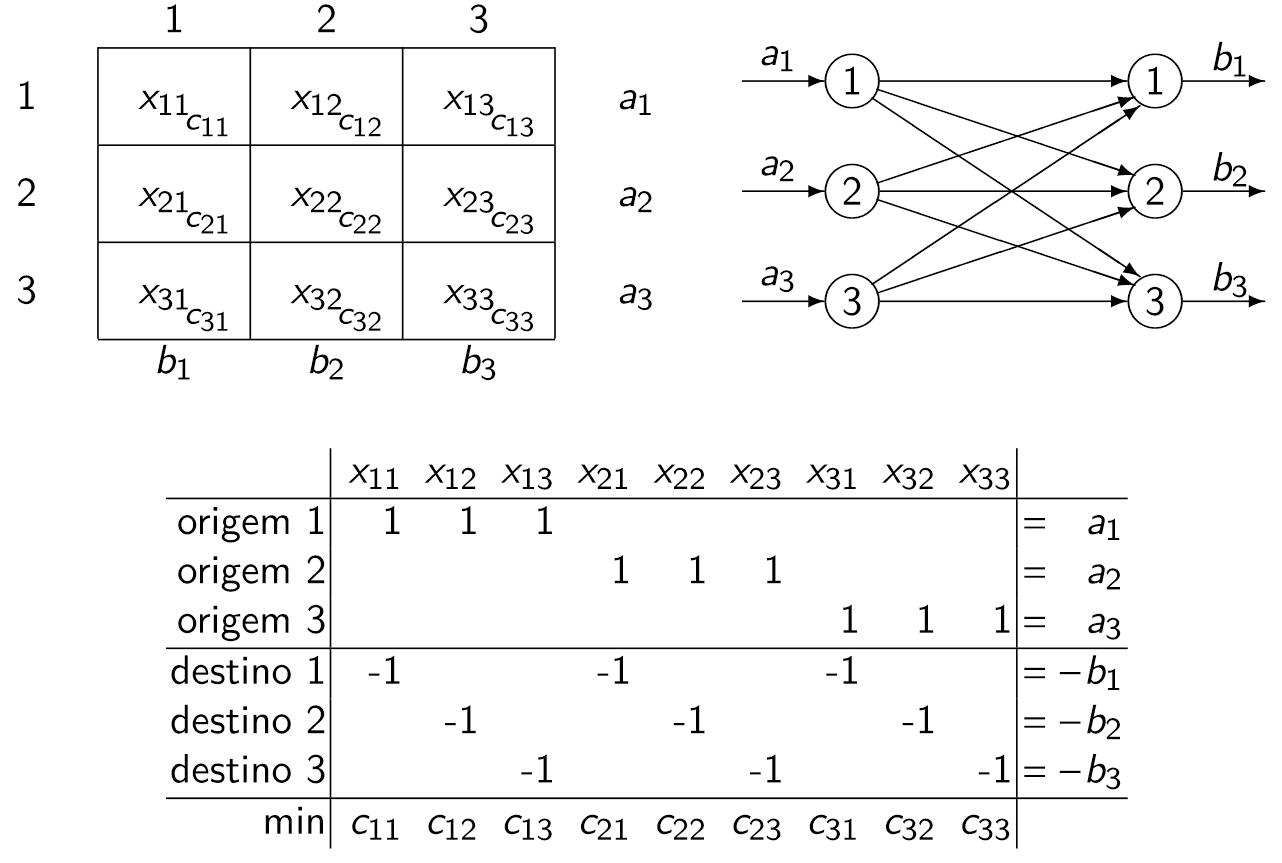
\includegraphics[width=0.45\textwidth]{bipartidos_repr.png}
%\end{figure}

\subsection{Solução inicial}

\subsubsection{Método do canto NW}

\begin{enumerate}
    \item Colocar a maior quantidade possível na casa mais a NW \(\implies\)
    \begin{itemize}
        \item ou a procura de um destino (coluna) é totalmente satisfeita,
        \item ou a oferta de uma origem (linha) é totalmente usada,
        \item ou ambas.
    \end{itemize}
    \item Cortar a linha ou a coluna (ou ambas)
    \item Repetir se ainda houver uma casa
\end{enumerate}

\subsubsection{Método do canto NW}

\begin{enumerate}
    \item Colocar a maior quantidade possível na casa com custo mínimo \(\implies\)
    \begin{itemize}
        \item ou a procura de um destino (coluna) é totalmente satisfeita,
        \item ou a oferta de uma origem (linha) é totalmente usada,
        \item ou ambas.
    \end{itemize}
    \item Cortar a linha ou a coluna (ou ambas)
    \item Repetir se ainda houver uma casa
\end{enumerate}

\subsubsection{Seleção da variável básica com valor 0 (quando faltar uma var. básica)}

\begin{figure}[H]
    \centering
    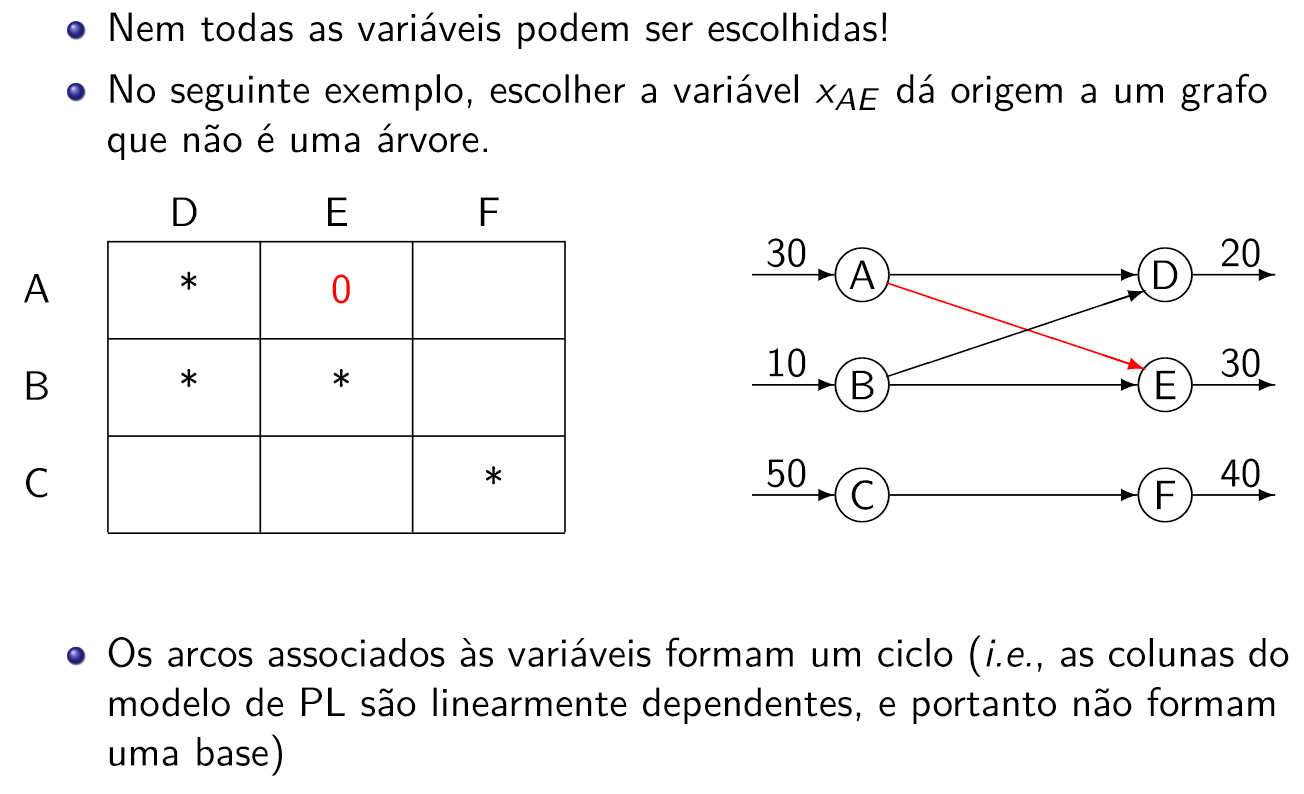
\includegraphics[width=0.45\textwidth]{var_basica_0.png}
\end{figure}

\subsection{Pivô}

\begin{figure}[H]
    \centering
    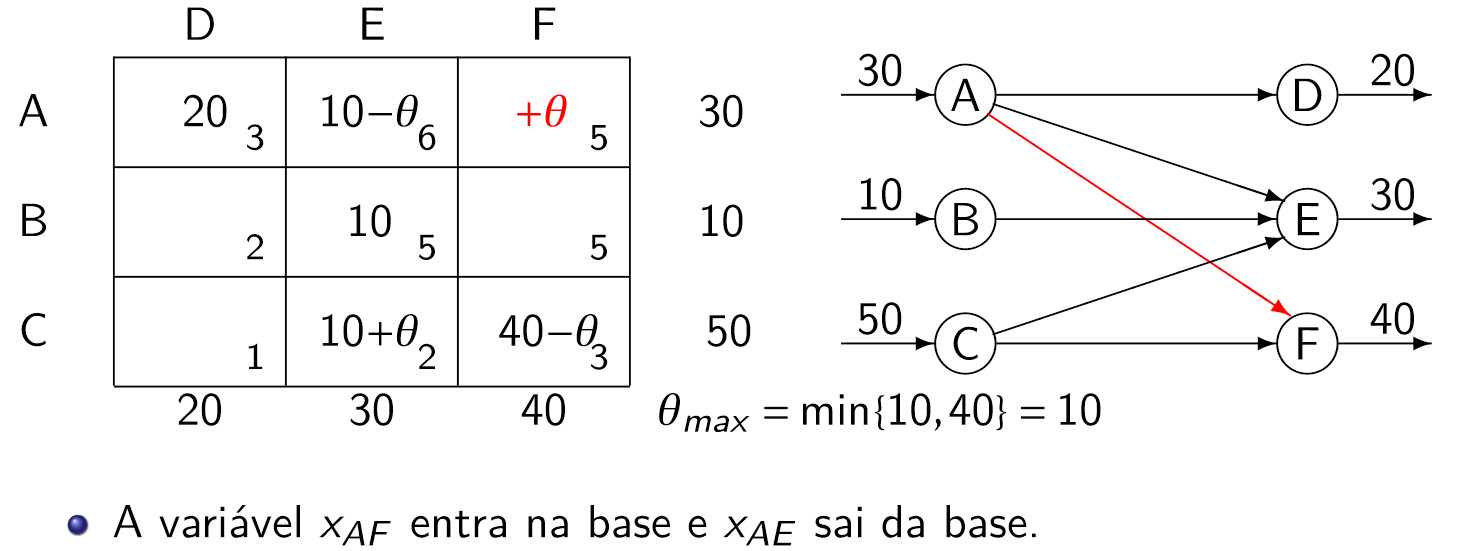
\includegraphics[width=0.45\textwidth]{bipartidos_pivo.png}
\end{figure}



%\section{Transportes: Redes sem capacidades}

%\dots (nada?)




\section{Transportes: Redes c/ capacidades}


\subsection{Caracterização das soluções básicas}

Iguais às referidas no 2.2, mas agora as variáveis no limite superior são também consideradas como não-básicas, para além das iguais a 0.

Uma variável não-básica é atrativa quando:
\begin{itemize}
    \item \(x_{ij} = 0\) (variável aumenta de valor) e \(\delta_{ij} < 0\)
    \item \(x_{ij} = u_{ij}\) (variável decrementa de valor) e \(\delta_{ij} > 0\)
\end{itemize}

\subsection{Transformações}

\subsubsection{Capacidade num vértice}

\begin{figure}[H]
    \centering
    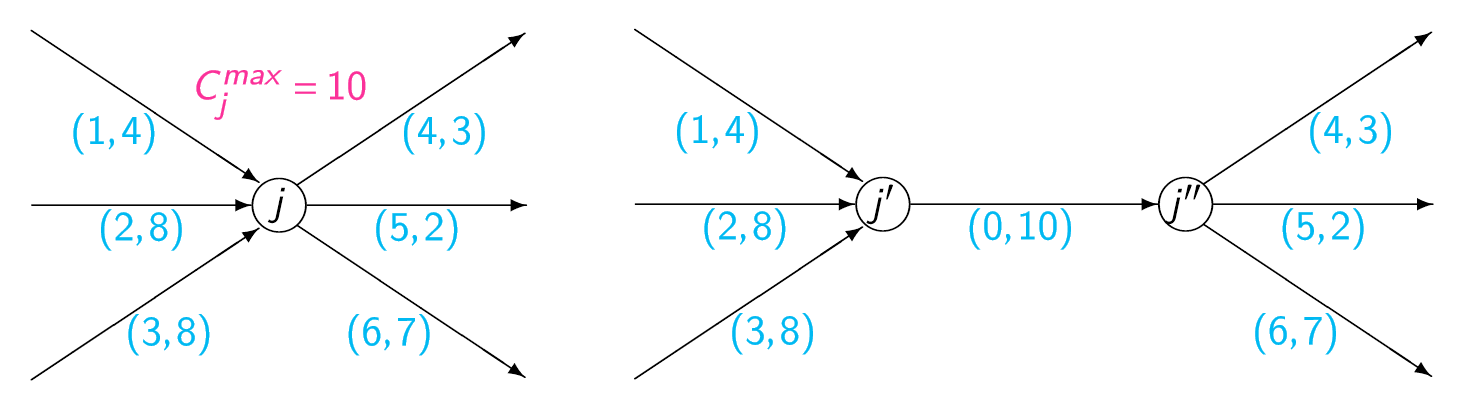
\includegraphics[width=0.45\textwidth]{cap_vertice.png}
\end{figure}

\subsubsection{Limite inferior num arco}

\begin{figure}[H]
    \centering
    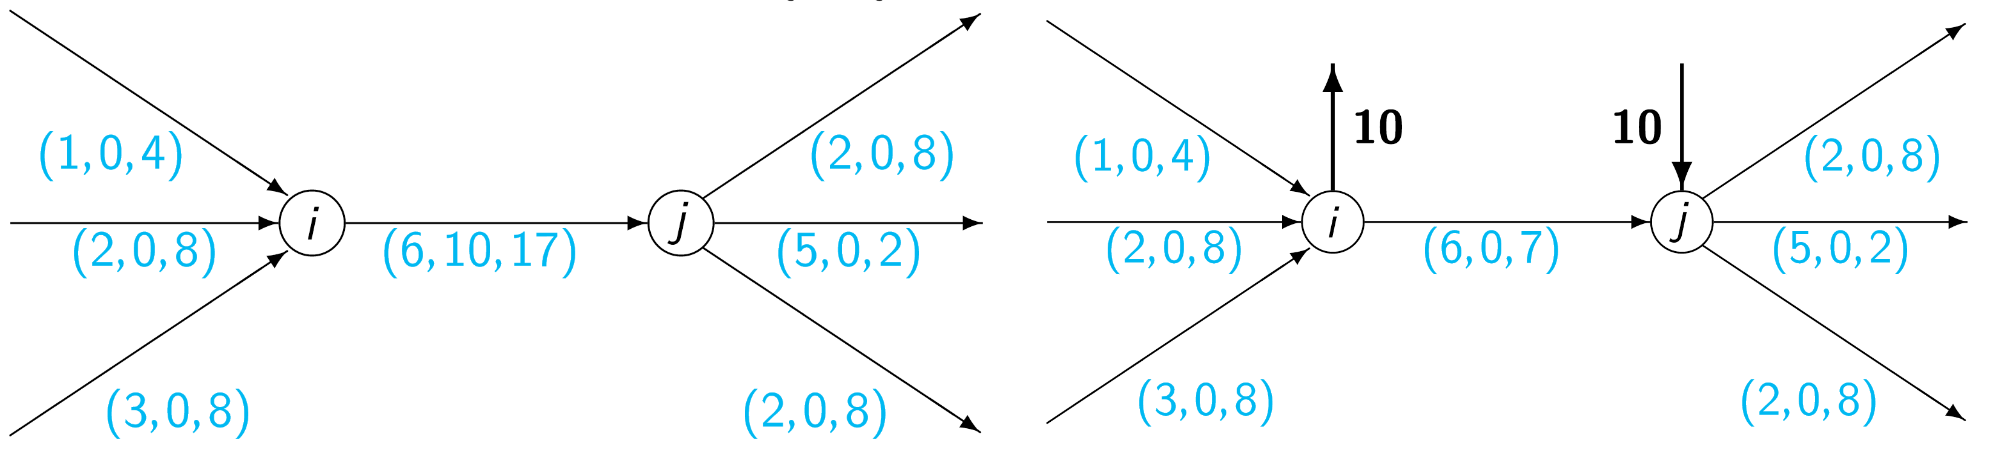
\includegraphics[width=0.45\textwidth]{limites.png}
\end{figure}



\section{Programação Inteira: Modelos}
\thispagestyle{empty}

\subsection{Expressões lógicas}

\begin{figure}[H]
    \centering
    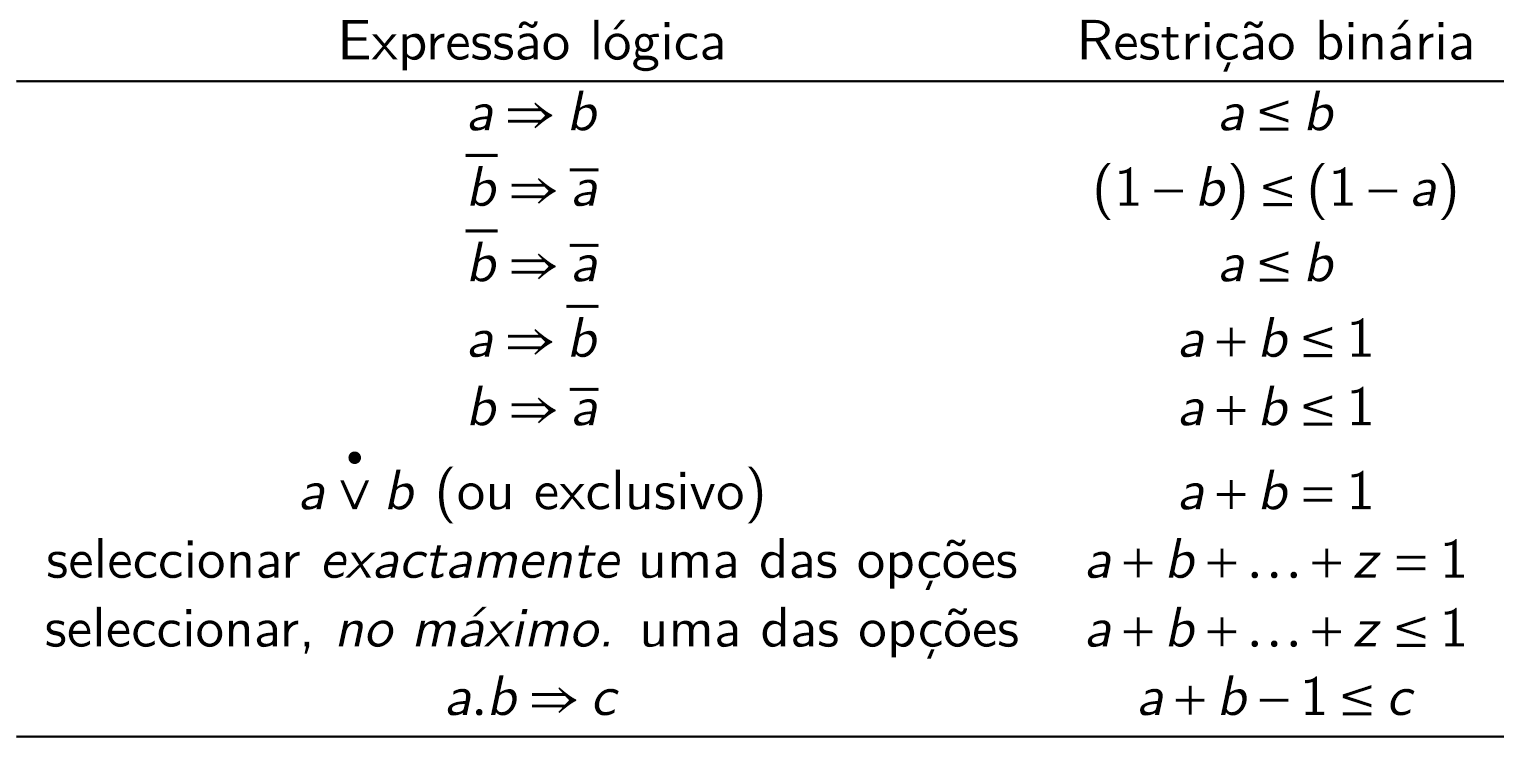
\includegraphics[width=0.45\textwidth]{expr_logicas.png}
\end{figure}


\section{PI: Planos de corte}

Estratégia do método dos planos de corte:
\begin{enumerate}
    \item determinar a solução óptima do problema de PL
    \item cortar partes do domínio em que não há sol. inteiras e reoptimizar, até obter uma sol. inteira (que é óptima!)
\end{enumerate}

\vspace{0.25cm}

Algoritmo de planos de corte:
\begin{enumerate}
    \item Optimizar \textit{relaxação linear}
    \item Enquanto a solução não for inteira:
    \begin{itemize}
        \item identificar um plano de corte
        \item adicionar plano de corte ao conjunto de restrições
        \item reoptimizar (usando o método simplex dual)
    \end{itemize}
\end{enumerate}



\section{PI: Partição e avaliação}

\subsection{Partição do domínio}

Dado um pai com uma solução fraccionária:
\begin{enumerate}
    \item selecionar variável \(x_j\) fraccionária
    \item criar 2 nós filhos, \(x_j \le \lfloor x_j \rfloor\) e \(x_j \ge \lceil x_j \rceil \)
\end{enumerate}

\subsection{Solução incumbente}

É a melhor solução inteira encontrada até um dado passo da pesquisa (\(x_\textsf{SI}\)) com valor de função objectivo \(z_\textsf{SI}\).

\subsection{Avaliação do nó (prob. maximização)}

\subsubsection{[Início] Determinar sol. ótima PL (\(x_\textsf{PL} \rightarrow z_\textsf{PL}\))}

\begin{itemize}
    \item se for inteira, é a melhor sol. inteira no domínio do nó
    \item se não, pode haver na subárvore uma sol. inteira \(\le z_\textsf{PL}\)
\end{itemize}

\subsubsection{[Opção 1] Abandonar o nó (podar a subárvore) se:}

\begin{itemize}
    \item o problema for impossível (domínio vazio)
    \item a solução \(x_\textsf{PL}\) for inteira (atualizar incumbente se \(z_\textsf{PL} > z_\textsf{SI}\))
    \item a solução \(x_\textsf{PL}\) for fraccionária e não puder haver na subárvore uma solução inteira melhor do que a solução incumbente \(z_\textsf{PL} \le z_\textsf{SI}\)
\end{itemize}

\subsubsection{[Opção 2] Fazer partição (explorar a subárvore):}

\begin{itemize}
    \item se a solução \(x_\textsf{PL}\) for fraccionária e ainda puder haver na subárvore uma solução inteira melhor do que a solução incumbente \(z_\textsf{PL} > z_\textsf{SI}\)
\end{itemize}

\subsection{Limites inf. e sup. para o valor do ótimo}

\(z_I^* \rightarrow\) solução ótima inteira

\[z_I^* \in [\textsf{LI}, \textsf{LS}]\]


\end{multicols}
\end{document}